% 2013 年北京卷文科第 17 题：四棱锥 P-ABCD。
% 来源 PDF：普通高考/2013/2013北京文.pdf，第 2 页（印面 790）左栏。
% AB∥CD，CD=2AB；PA⊥底面，A 在图中为被遮住的顶点，故 PA、AB、AD 画虚线；
% E 为 CD 中点，F 为 PC 中点，BE 在底面内被遮挡画虚线，BF、FE 画实线。
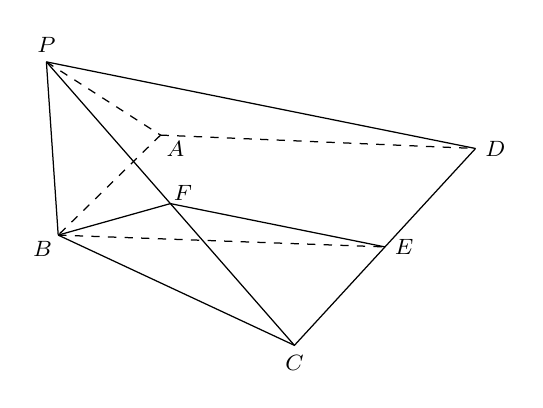
\begin{tikzpicture}[font=\footnotesize, line width=0.45pt]
  \coordinate (P) at (1.40,3.85);
  \coordinate (A) at (2.85,2.92);
  \coordinate (B) at (1.55,1.65);
  \coordinate (C) at (4.55,0.25);
  \coordinate (D) at (6.85,2.75);
  \coordinate (E) at (5.70,1.50);
  \coordinate (F) at (2.975,2.05);
  % 可见棱
  \draw (P) -- (B);
  \draw (P) -- (C);
  \draw (P) -- (D);
  \draw (B) -- (C) -- (D);
  \draw (B) -- (F) -- (E);
  % 被遮挡的棱
  \draw[dashed] (P) -- (A);
  \draw[dashed] (A) -- (B);
  \draw[dashed] (A) -- (D);
  \draw[dashed] (B) -- (E);
  % 顶点标注
  \node[above] at (P) {$P$};
  \node[below right, inner sep=2pt] at (A) {$A$};
  \node[below left, inner sep=2pt] at (B) {$B$};
  \node[below] at (C) {$C$};
  \node[right] at (D) {$D$};
  \node[right] at (E) {$E$};
  \node[above right, inner sep=1pt] at (F) {$F$};
\end{tikzpicture}
